\documentclass[conference]{IEEEtran}
\IEEEoverridecommandlockouts
\usepackage{cite}
\usepackage{amsmath,amssymb,amsfonts}
\usepackage{graphicx}
\usepackage{textcomp}
\usepackage{xcolor}
\usepackage{booktabs}
\usepackage{tikz}
\usetikzlibrary{arrows.meta,positioning,fit,backgrounds}
\usepackage[hyphens]{url}
\usepackage[colorlinks=true,linkcolor=black,citecolor=black,urlcolor=blue!55!black]{hyperref}
\graphicspath{{figures/}{../../results/figures/}}
% Colour tokens shared by the diagrams (same hues as the plots).
\definecolor{diagInk}{HTML}{1F2A44}
\definecolor{diagGrey}{HTML}{F1F0EC}
\definecolor{diagBlue}{HTML}{2A78D6}
\definecolor{diagOrange}{HTML}{EB6834}
\definecolor{diagGreen}{HTML}{1BAF7A}
\definecolor{diagYellow}{HTML}{EDA100}

\renewcommand{\topfraction}{0.9}
\renewcommand{\dbltopfraction}{0.9}
\renewcommand{\textfraction}{0.07}
\renewcommand{\floatpagefraction}{0.75}
\renewcommand{\dblfloatpagefraction}{0.75}

\begin{document}

\title{Speech-to-Action: A Comparative Study of Classical and Deep Learning Approaches for Spoken Intent Classification}

\author{\IEEEauthorblockN{Shruti Sivakumar}
\IEEEauthorblockA{\textit{Amrita School of Artificial Intelligence} \\
\textit{Amrita Vishwa Vidyapeetham}\\
Coimbatore, India \\
CB.SC.U4AIE23254}
\and
\IEEEauthorblockN{Vida Nadheera S}
\IEEEauthorblockA{\textit{Amrita School of Artificial Intelligence} \\
\textit{Amrita Vishwa Vidyapeetham}\\
Coimbatore, India \\
CB.SC.U4AIE23244}
\and
\IEEEauthorblockN{Shreya Sriram}
\IEEEauthorblockA{\textit{Amrita School of Artificial Intelligence} \\
\textit{Amrita Vishwa Vidyapeetham}\\
Coimbatore, India \\
CB.SC.U4AIE23248}
}

\maketitle

\begin{abstract}
Spoken intent classification is the task of finding the action that a short voice command asks for. Most of the recent work on this task uses large pre-trained models, so it is not clear how much each type of speech representation actually contributes. To understand this, this study was conducted on the Fluent Speech Commands corpus, which has 30,043 utterances from 97 speakers and 31 intents. First, a classical feature-extraction pipeline (short-time energy, zero-crossing rate, autocorrelation pitch, linear prediction and mel-frequency cepstral coefficients, or MFCC) was built and checked on individual utterances. These features were summarised over each utterance and classified using a support vector machine (SVM) and a multilayer perceptron. Dynamic time warping and per-class Gaussian hidden Markov models were used as classical sequence baselines. After this, one-dimensional convolutional networks were trained from scratch on MFCC and log-mel sequences, and a frozen wav2vec~2.0 encoder was tested with pooled and frame-sequence classifiers. All the models were compared using five-fold speaker-grouped cross-validation, on the 31-class task and also on reduced-class tasks for the action, object and location slots. The utterance statistics reach $24.0 \pm 1.0\%$ on the intent and stay close to the majority-class baseline on the slot tasks. A convolutional network on log-mel sequences reaches $79.4 \pm 6.8\%$. When the cepstral DCT is applied to the same input, this drops to $63.5\%$, because per-channel standardisation gives too much weight to the low-variance coefficients. The same network on frozen wav2vec~2.0 frames reaches $93.1 \pm 3.1\%$ on the intent and 95.1--97.5\% on the slots. From this, it is clear that keeping the temporal order of the utterance matters more than changing the static features or reducing the number of classes. The errors that remain in the best model are mostly between commands of opposite polarity.
\end{abstract}

\begin{IEEEkeywords}
spoken language understanding, intent classification, linear prediction, MFCC, dynamic time warping, hidden Markov model, convolutional neural network, wav2vec 2.0
\end{IEEEkeywords}

%=====================================================================
\section{Introduction}
%=====================================================================
Voice assistants at home are usually given short commands such as \emph{``turn the kitchen lights off''} or \emph{``make the music louder''}. To carry out such a command, the device does not need a transcript of what was said; it only needs to know the action. Spoken language understanding (SLU) systems have traditionally done this in two steps. A speech recogniser first converts the audio to text, and a text classifier then finds the intent. End-to-end SLU models skip the transcript and map the audio directly to the intent~\cite{serdyuk2018e2eslu,lugosch2019fsc}. The Fluent Speech Commands (FSC) corpus~\cite{lugosch2019fsc} was released for this end-to-end approach. Today, most of the results reported on it come from models that are pre-trained on large amounts of speech~\cite{lugosch2019fsc,radfar2020transformer,yang2021superb}.

Since the accuracies on FSC are already very high, a different question has not been looked at as much. How much of the task is solved by each type of speech representation, starting from the short-time measurements of classical speech analysis and going up to the embeddings of a self-supervised encoder? To answer this, the representation has to be changed while the classifier and the evaluation are kept the same as far as possible. Hence, this study is organised into four tiers. The first tier uses hand-crafted features that are summarised over the whole utterance. The second tier applies classical sequence models, namely dynamic time warping and hidden Markov models, to MFCC sequences. The third tier trains convolutional networks from scratch on MFCC and log-mel sequences. The fourth tier uses the same convolutional network on top of a frozen wav2vec~2.0 encoder~\cite{baevski2020wav2vec2}.

The main contributions of this work are:
\begin{itemize}
\item A classical feature-extraction pipeline (energy, zero-crossing rate, autocorrelation pitch, short-time Fourier analysis and linear prediction) is implemented and checked on a single utterance. It is then used to measure how much accuracy prosodic statistics alone can give on FSC.
\item Four representation tiers are compared under the same conditions. This includes classical sequence baselines, and an ablation that separates the two effects of the cepstral DCT (decorrelation and truncation) while the convolutional network is kept the same.
\item It is shown that the official FSC splits have too few speakers for a reliable evaluation on one split. Five-fold speaker-grouped cross-validation, with paired comparisons across folds, is used instead.
\item Reduced-class tasks based on the slots of the labels (action, object and location) are evaluated along with the 31-class task. The errors of the best model are also analysed, in terms of how the commands are phrased and how the speakers differ.
\end{itemize}

The rest of this paper is organised as follows. Section~\ref{sec:related} reviews the related work, and Section~\ref{sec:gaps} gives the research gaps and objectives. Section~\ref{sec:data} describes the dataset and Section~\ref{sec:method} explains the methodology. The results are discussed in Section~\ref{sec:results}, and Section~\ref{sec:conclusion} concludes the paper.

%=====================================================================
\section{Related Work}\label{sec:related}
%=====================================================================
\subsection{Short-time analysis and classical features}
Short-time energy and zero-crossing rate were used together by Rabiner and Sambur~\cite{rabiner1975endpoints} to find the start and end points of isolated words. Atal and Rabiner~\cite{atal1976vus} then treated the voiced/unvoiced/silence decision as a pattern classification problem, using several of these measurements together. Pitch detection using autocorrelation was analysed by Rabiner~\cite{rabiner1977pitch}, who also limited the range of lags that are searched so that octave errors are reduced. The YIN estimator~\cite{decheveigne2002yin} later reduced these errors further using a cumulative mean-normalised difference function. Short-time Fourier analysis and synthesis was formalised by Allen and Rabiner~\cite{allen1977stft}. Linear prediction was explained in detail by Makhoul~\cite{makhoul1975lp}; in this method, the autocorrelation equations are solved using the Levinson--Durbin recursion. Mel-frequency cepstral coefficients were introduced by Davis and Mermelstein~\cite{davis1980mfcc}, who showed that they work better than linear prediction parameters for word recognition. Furui~\cite{furui1986delta} showed that time-derivative cepstral features are useful for speaker-independent recognition.

\subsection{Classical sequence modelling}
Dynamic time warping (DTW) was introduced by Sakoe and Chiba~\cite{sakoe1978dtw} to align utterances of different lengths with stored templates. The hidden Markov model (HMM) became the standard statistical model for speech of variable length after Rabiner's tutorial~\cite{rabiner1989hmm}, with Gaussian emission densities over the cepstral frames. Both of these methods were made for isolated-word recognition with small vocabularies. This is quite similar to classifying commands.

\subsection{Neural acoustic models and the choice of input feature}
When deep networks started being used for acoustic modelling~\cite{hinton2012dnn}, the role of feature extraction also changed. Mohamed \emph{et al.}~\cite{mohamed2012understanding} found that deep belief networks work better on log mel filter-bank energies than on MFCC. According to them, this is because the cepstral transform loses some information, and because the network can handle correlated inputs on its own. Abdel-Hamid \emph{et al.}~\cite{abdelhamid2014cnn} applied convolution along the frequency and time axes of filter-bank inputs. Sainath and Parada~\cite{sainath2015kws} showed that small convolutional networks work well for keyword spotting, even with limited computation. The Speech Commands corpus~\cite{warden2018speechcommands} gave a standard benchmark for recognising short commands like these. SpecAugment~\cite{park2019specaugment} introduced time and frequency masking as a way of augmenting the input features. Studies that compare feature types in other speech classification tasks~\cite{devi2021meeteilon,nanmalar2025tamil} also found that a single type of hand-crafted feature stops improving after a point, and that cepstral features or a combination of features recover much of the gap.

\subsection{End-to-end SLU and self-supervised representations}
Serdyuk \emph{et al.}~\cite{serdyuk2018e2eslu} showed that intent can be predicted directly from audio without a transcript in between. FSC was released by Lugosch \emph{et al.}~\cite{lugosch2019fsc} along with a model whose lower layers are pre-trained to recognise phonemes and words. This model gets 98.8\% accuracy when the pre-trained layers are frozen, and 96.6\% when it is trained from random initialisation. Radfar \emph{et al.}~\cite{radfar2020transformer} reported 99.6\% intent accuracy using an end-to-end transformer. Self-supervised encoders learn speech representations from audio that has no labels~\cite{schneider2019wav2vec,baevski2020wav2vec2,hsu2021hubert}. For example, wav2vec~2.0~\cite{baevski2020wav2vec2} masks parts of its latent speech features and solves a contrastive task over quantised targets. The SUPERB benchmark~\cite{yang2021superb} tests frozen encoders with small task-specific heads. On FSC, it reports intent accuracies of 9.10\% for log mel filter-bank input, 92.35\% for wav2vec~2.0 Base and 98.34\% for HuBERT Base. Pasad \emph{et al.}~\cite{pasad2021layerwise} also showed that phonetic and word information is not spread evenly across the layers of wav2vec~2.0. The published FSC results that are used for comparison in Section~\ref{sec:results} are listed in Table~\ref{tab:lit}.

\begin{table}[t]
\caption{Published intent accuracy on FSC (official test split)}
\label{tab:lit}
\centering
\footnotesize
\begin{tabular}{@{}llr@{}}
\toprule
Work & Model & Acc. (\%)\\
\midrule
SUPERB~\cite{yang2021superb} & Log mel filter bank, frozen & 9.10\\
SUPERB~\cite{yang2021superb} & wav2vec 2.0 Base, frozen & 92.35\\
SUPERB~\cite{yang2021superb} & HuBERT Base, frozen & 98.34\\
Lugosch \emph{et al.}~\cite{lugosch2019fsc} & End-to-end, no pre-training & 96.6\\
Lugosch \emph{et al.}~\cite{lugosch2019fsc} & ASR pre-trained, frozen & 98.8\\
Radfar \emph{et al.}~\cite{radfar2020transformer} & End-to-end transformer & 99.6\\
\bottomrule
\end{tabular}
\end{table}

%=====================================================================
\section{Research Gaps and Objectives}\label{sec:gaps}
%=====================================================================
From the literature reviewed above, the following gaps were identified:
\begin{enumerate}
\item Work on FSC is mostly based on pre-trained end-to-end models~\cite{lugosch2019fsc,radfar2020transformer,yang2021superb}. The accuracy that classical, interpretable speech features can reach on this corpus is rarely reported.
\item Cepstral features are known to do better than prosodic or formant features for word recognition~\cite{davis1980mfcc}. However, this gap has not been measured for an intent task with the classifier kept fixed.
\item Classical sequence models such as DTW and HMM~\cite{sakoe1978dtw,rabiner1989hmm} and neural sequence models~\cite{abdelhamid2014cnn,sainath2015kws} are rarely compared on the same input features without pre-training.
\item The effect of the cepstral (DCT) step on a convolutional classifier has been studied for acoustic modelling~\cite{mohamed2012understanding}, but not for classifying the intent of a whole utterance.
\item The published FSC results use the official test split, which has only ten speakers. How much these results depend on the choice of speakers is not reported.
\end{enumerate}

Based on these gaps, the objectives of this study are:
\begin{enumerate}
\item to implement and verify a classical feature-extraction pipeline based on short-time analysis, and to measure the intent accuracy of prosodic and cepstral utterance statistics with SVM and MLP classifiers;
\item to test DTW and Gaussian HMM classifiers on MFCC sequences;
\item to train convolutional sequence models from scratch on MFCC and log-mel inputs, including a multi-head model that follows the slot structure of the labels;
\item to evaluate a frozen wav2vec~2.0 representation with pooled and sequence-level classifiers;
\item to repeat the evaluation on reduced-class slot tasks with 4, 6 and 14 classes; and
\item to compare all the models using speaker-grouped cross-validation and to analyse the errors that remain.
\end{enumerate}

%=====================================================================
\section{Dataset}\label{sec:data}
%=====================================================================
The Fluent Speech Commands corpus~\cite{lugosch2019fsc} is used in this study. It has 30,043 English utterances (19.0~h) recorded at 16~kHz by 97 speakers. Each utterance is labelled with three slots: \emph{action} (6 values), \emph{object} (14 values) and \emph{location} (4 values). The combinations of these slots that occur in the data make up 31 intents, and these intents are spoken using 248 different phrasings. The official split is speaker-independent (Table~\ref{tab:data}). Before running any experiment, it was confirmed that no speaker appears in more than one subset. The corpus is released under a non-commercial licence for academic research.

\begin{table}[t]
\caption{Official FSC partition}
\label{tab:data}
\centering
\footnotesize
\begin{tabular}{@{}lrr@{}}
\toprule
Subset & Utterances & Speakers\\
\midrule
Train & 23,132 & 77\\
Validation & 3,118 & 10\\
Test & 3,793 & 10\\
\midrule
Total & 30,043 & 97\\
\bottomrule
\end{tabular}
\end{table}

The intents are not equally represented (Fig.~\ref{fig:intents}). The two volume commands have 2,296 and 2,099 training utterances, while the rarest intents have only 342--401. Hence, a classifier that always predicts the most common class already gets 10.4\% on the test subset. On average, an utterance is 2.31~s long, and 95\% of the utterances are shorter than 3.41~s. Two things about this corpus are important for the analysis later on. First, some intents differ only in the polarity of the action, and this polarity is often decided by one short word, such as \emph{``turn the lamp on''} and \emph{``turn the lamp off''}, or \emph{``volume up''} and \emph{``volume down''}. Second, the official validation and test subsets have only ten speakers each.

\begin{figure}[t]
\centering
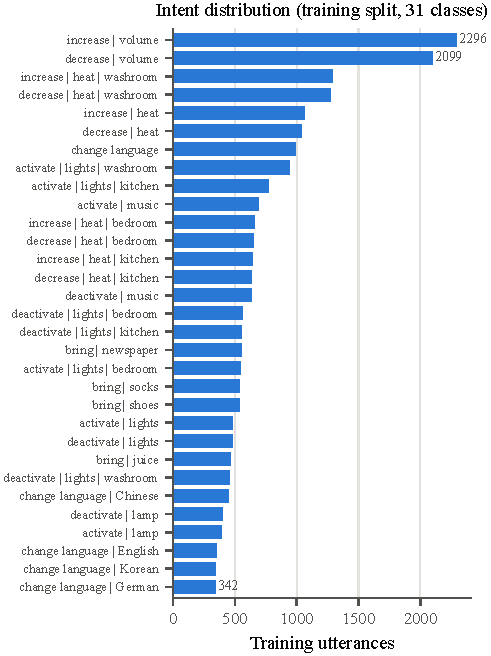
\includegraphics[width=\columnwidth]{fig_intent_dist.pdf}
\caption{Number of training utterances per intent (action~\textbar~object~\textbar~location; the value \emph{none} is not shown).}
\label{fig:intents}
\end{figure}

%=====================================================================
\section{Methodology}\label{sec:method}
%=====================================================================
The overall procedure is shown in Fig.~\ref{fig:flow}. All four tiers use the same input, labels and evaluation metric. They differ only in how the utterance is represented and which classifier is used on it.

\begin{figure*}[t]
\centering
\resizebox{0.97\textwidth}{!}{% Methodology flow diagram (shared by the report and the slides).
% Requires: tikz with arrows.meta, positioning, fit, backgrounds.
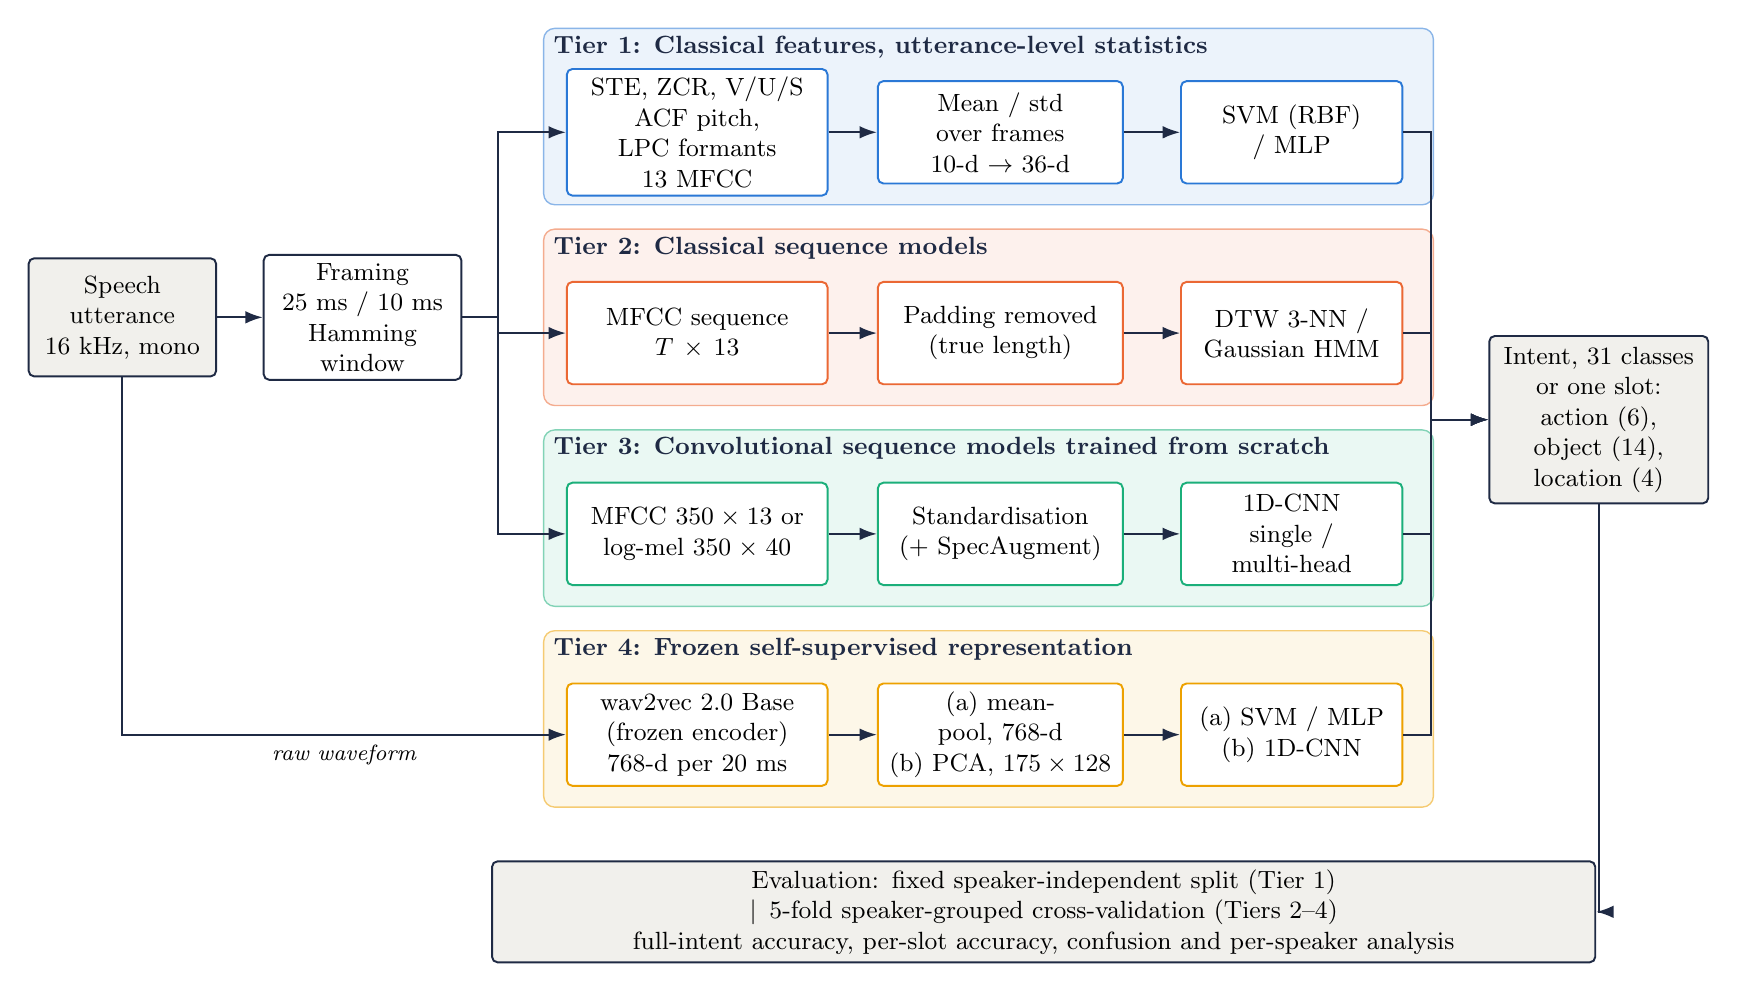
\begin{tikzpicture}[
  font=\small, >={Latex[length=2.2mm,width=1.6mm]},
  box/.style={draw=#1, fill=white, rounded corners=2pt, line width=0.7pt, align=center,
              minimum height=1.3cm, inner sep=3pt},
  io/.style={draw=diagInk, fill=diagGrey, rounded corners=2pt, line width=0.7pt, align=center,
             minimum height=1.5cm, inner sep=4pt},
  band/.style={fill=#1!9, draw=#1!55, rounded corners=4pt, line width=0.5pt},
  tier/.style={font=\small\bfseries, anchor=north west, text=diagInk, inner sep=2pt},
  arr/.style={->, line width=0.7pt, draw=diagInk},
]
% ---------------- tier bands ----------------
\def\tierA{5.1} \def\tierB{2.55} \def\tierC{0.0} \def\tierD{-2.55}
\foreach \y/\c/\t in {\tierA/diagBlue/{Tier 1: Classical features, utterance-level statistics},
                      \tierB/diagOrange/{Tier 2: Classical sequence models},
                      \tierC/diagGreen/{Tier 3: Convolutional sequence models trained from scratch},
                      \tierD/diagYellow/{Tier 4: Frozen self-supervised representation}}{
  \fill[band=\c] (5.05,\y-1.12) rectangle (16.35,\y+1.12);
  \node[tier] at (5.1,\y+1.1) {\t};
}
% ---------------- input and pre-processing ----------------
\node[io, text width=2.1cm] (in) at (-0.3,\tierB) {Speech utterance\\16 kHz, mono};
\node[box=diagInk, text width=2.3cm, minimum height=1.5cm] (pre) at (2.75,\tierB)
     {Framing\\25 ms / 10 ms\\Hamming window};
% ---------------- Tier 1 ----------------
\node[box=diagBlue, text width=3.1cm] (a1) at (7.0,\tierA-0.2) {STE, ZCR, V/U/S\\ACF pitch, LPC formants\\13 MFCC};
\node[box=diagBlue, text width=2.9cm] (a2) at (10.85,\tierA-0.2) {Mean / std\\over frames\\10-d $\rightarrow$ 36-d};
\node[box=diagBlue, text width=2.6cm] (a3) at (14.55,\tierA-0.2) {SVM (RBF) / MLP};
% ---------------- Tier 2 ----------------
\node[box=diagOrange, text width=3.1cm] (b1) at (7.0,\tierB-0.2) {MFCC sequence\\$T \times 13$};
\node[box=diagOrange, text width=2.9cm] (b2) at (10.85,\tierB-0.2) {Padding removed\\(true length)};
\node[box=diagOrange, text width=2.6cm] (b3) at (14.55,\tierB-0.2) {DTW 3-NN /\\Gaussian HMM};
% ---------------- Tier 3 ----------------
\node[box=diagGreen, text width=3.1cm] (c1) at (7.0,\tierC-0.2) {MFCC $350 \times 13$ or\\log-mel $350 \times 40$};
\node[box=diagGreen, text width=2.9cm] (c2) at (10.85,\tierC-0.2) {Standardisation\\(+ SpecAugment)};
\node[box=diagGreen, text width=2.6cm] (c3) at (14.55,\tierC-0.2) {1D-CNN\\single / multi-head};
% ---------------- Tier 4 ----------------
\node[box=diagYellow, text width=3.1cm] (d1) at (7.0,\tierD-0.2) {wav2vec 2.0 Base\\(frozen encoder)\\768-d per 20 ms};
\node[box=diagYellow, text width=2.9cm] (d2) at (10.85,\tierD-0.2) {(a) mean-pool, 768-d\\(b) PCA, $175 \times 128$};
\node[box=diagYellow, text width=2.6cm] (d3) at (14.55,\tierD-0.2) {(a) SVM / MLP\\(b) 1D-CNN};
% ---------------- output and evaluation ----------------
\node[io, text width=2.5cm] (out) at (18.45,1.25) {Intent, 31 classes\\or one slot:\\action (6), object (14),\\location (4)};
\node[box=diagInk, fill=diagGrey, text width=13.8cm, minimum height=0.95cm] (ev) at (11.4,-5.0)
     {Evaluation: fixed speaker-independent split (Tier 1) \,$\vert$\, 5-fold speaker-grouped cross-validation (Tiers 2--4)\\
      full-intent accuracy, per-slot accuracy, confusion and per-speaker analysis};
% ---------------- arrows ----------------
\draw[arr] (in) -- (pre);
\foreach \n in {a1,b1,c1}{ \draw[arr] (pre.east) -- ++(0.45,0) |- (\n.west); }
\draw[arr] (in.south) |- node[pos=0.75, below, font=\footnotesize\itshape] {raw waveform} (d1.west);
\foreach \p/\q in {a1/a2,a2/a3,b1/b2,b2/b3,c1/c2,c2/c3,d1/d2,d2/d3}{ \draw[arr] (\p) -- (\q); }
\foreach \n in {a3,b3,c3,d3}{ \draw[arr] (\n.east) -- ++(0.35,0) |- (out.west); }
\draw[arr] (out.south) |- (ev.east);
\end{tikzpicture}
}
\caption{Methodology. The four tiers go from classical to modern representations; each tier gives an intent decision, which is evaluated using the protocol shown at the bottom.}
\label{fig:flow}
\end{figure*}

\subsection{Pre-processing and short-time analysis}
Each signal $x[n]$ is divided into frames of $N = 400$ samples (25~ms) with a hop of 160 samples (10~ms). Each frame is then multiplied by the Hamming window
\begin{equation}
w[n] = 0.54 - 0.46\cos\!\left(\frac{2\pi n}{N-1}\right), \quad 0 \le n \le N-1 .
\end{equation}
For frame $m$ with samples $x_m[n]$, the short-time energy and the zero-crossing rate are
\begin{align}
E_m &= \sum_{n=0}^{N-1} x_m^2[n], \\
Z_m &= \frac{1}{N-1}\sum_{n=1}^{N-1} \tfrac{1}{2}\left|\operatorname{sgn}(x_m[n]) - \operatorname{sgn}(x_m[n-1])\right| .
\end{align}
A frame is labelled as speech if $10\log_{10}E_m$ is more than 10~dB above the 15th percentile of the frame energies in that utterance. Among the speech frames, a frame is labelled unvoiced if its $Z_m$ is above the 70th percentile of $Z$, and voiced otherwise. So both thresholds depend on the recording itself. This is needed because the signal level is different for each speaker, microphone and recording gain, and there are 97 speakers in the corpus.

For the voiced frames, the short-time autocorrelation $r_m[k] = \sum_{n} x_m[n]\,x_m[n+k]$ is calculated, and its highest peak is found within the lags that correspond to 70--400~Hz. The fundamental frequency is then $F_0 = f_s/k^{\ast}$. The ratio $r_m[k^{\ast}]/r_m[0]$ is used as a voicing confidence, and any estimate below 0.3 is treated as unreliable. Spectrograms are calculated as the squared magnitude of the short-time Fourier transform~\cite{allen1977stft}. In linear prediction, each sample is predicted as $\hat{x}[n] = -\sum_{k=1}^{p} a_k x[n-k]$. The coefficients for order $p = 16$ are found from the autocorrelation of the windowed frame using the Levinson--Durbin recursion~\cite{makhoul1975lp}. The formants are taken as the peaks of $1/|A(e^{j\omega})|$ below 3.5~kHz that have a prominence of at least 0.3~dB. The prediction residual $e[n] = x[n]-\hat{x}[n]$ gives an approximate form of the excitation. MFCCs~\cite{davis1980mfcc} are calculated from the same frames using a mel filter bank, a logarithm and a discrete cosine transform (DCT), and the first 13 coefficients are kept.

\subsection{Tier 1: utterance-level statistics}
Each utterance is summarised using ten prosodic statistics. These are the mean and standard deviation of the frame energy (in dB), of the zero-crossing rate and of $F_0$; the fraction of frames that are voiced; the mean of the first and second formant frequencies over the voiced frames; and the duration. To process the full corpus, $F_0$ is estimated with the YIN algorithm~\cite{decheveigne2002yin}. YIN uses the same idea of periodicity as the autocorrelation method, but it is much faster. When the mean and standard deviation of each of the 13 MFCCs are added, a 36-dimensional vector is obtained. All the features are standardised using the statistics of the training set. An RBF-kernel SVM~\cite{cortes1995svm} is tuned over $C \in \{1, 10, 100\}$ and $\gamma \in \{\text{scale}, 0.01, 0.1\}$, and an MLP is tuned over hidden layers $\{(64), (128), (64, 32)\}$ and $L_2$ penalty $\alpha \in \{10^{-4}, 10^{-3}\}$. The best setting is selected on the official validation subset. Inverse-frequency class weighting was also tried. The selected settings are evaluated again later, without any changes, using the cross-validation protocol in Section~\ref{sec:protocol}.

\subsection{Tier 2: classical sequence models}
For storage, the MFCC sequences are padded or cut to 350 frames, which is the 95th percentile of the duration. However, the padding is removed before sequence modelling, so that each model only sees the actual length of the utterance. For DTW~\cite{sakoe1978dtw}, an approximate multiscale DTW with Euclidean distance is used. Each query is compared with five randomly picked templates per intent (155 in total), and the label is decided by a 3-nearest-neighbour vote. Since each comparison takes a lot of time, DTW is evaluated on 155 queries (five per intent) taken from the held-out speakers of the first cross-validation fold. For the HMM~\cite{rabiner1989hmm}, one three-state Gaussian HMM with diagonal covariances is trained for each intent, using 20 Baum--Welch iterations. A query is given the intent whose model gives the highest log-likelihood.

\subsection{Tier 3: convolutional sequence models}
The convolutional network in Fig.~\ref{fig:cnn} works along the time axis, and the feature dimensions are treated as channels. It is trained from random initialisation with Adam~\cite{kingma2014adam} and sparse categorical cross-entropy, with a batch size of 128 and up to 50 epochs. Training is stopped early (patience of 8 epochs) based on a separate validation group of speakers. The inputs are standardised for each channel using statistics from the training fold. The input representation is changed first, and then the output structure:
\begin{enumerate}
\item[(i)] a single 31-way output is trained on 13-dimensional MFCC sequences (115,871 parameters);
\item[(ii)] the same network is trained on 40-band log-mel sequences with the same framing. The only difference from MFCC is that the DCT, and the truncation after it, are not applied;
\item[(iii)] to separate these two steps, the orthonormal DCT-II is applied to the same 40-band log-mel frames, and either all 40 coefficients (an invertible transform) or only the first 13 are kept;
\item[(iv)] lastly, the output is split into slots. In this multi-head model, a shared network on MFCC input feeds three softmax layers for the action, object and location. It is trained with the sum of the three losses and with SpecAugment-style masking~\cite{park2019specaugment} of two 20-frame time blocks and two 3-coefficient blocks per sequence.
\end{enumerate}
A multi-head prediction is counted as correct only if all three slots are correct.

\begin{figure*}[t]
\centering
\resizebox{0.92\textwidth}{!}{% 1D-CNN used for every sequence experiment (Tiers 3 and 4).
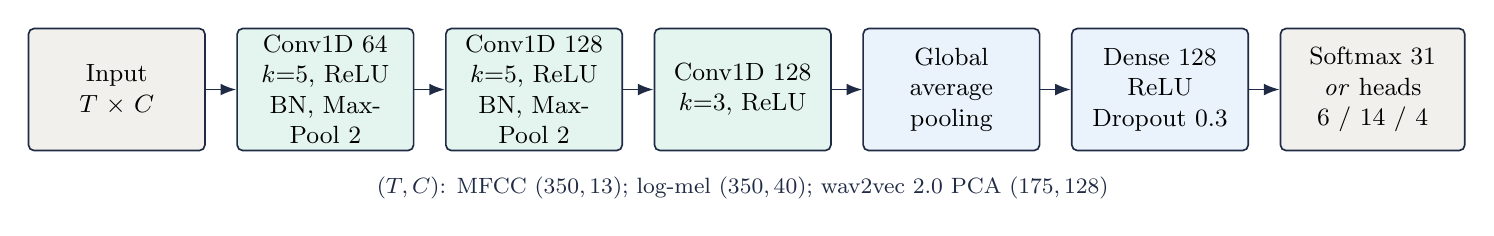
\begin{tikzpicture}[
  font=\small, >={Latex[length=2mm,width=1.5mm]},
  layer/.style={draw=diagInk, fill=#1, rounded corners=2pt, line width=0.6pt, align=center,
                minimum height=1.55cm, text width=2.1cm, inner sep=2pt},
  arr/.style={->, line width=0.7pt, draw=diagInk},
]
\node[layer=diagGrey] (x) at (0,0) {Input\\$T \times C$};
\node[layer=diagGreen!12] (c1) at (2.65,0) {Conv1D 64\\$k{=}5$, ReLU\\BN, MaxPool 2};
\node[layer=diagGreen!12] (c2) at (5.30,0) {Conv1D 128\\$k{=}5$, ReLU\\BN, MaxPool 2};
\node[layer=diagGreen!12] (c3) at (7.95,0) {Conv1D 128\\$k{=}3$, ReLU};
\node[layer=diagBlue!10] (g) at (10.60,0) {Global\\average\\pooling};
\node[layer=diagBlue!10] (d) at (13.25,0) {Dense 128\\ReLU\\Dropout 0.3};
\node[layer=diagGrey, text width=2.2cm] (o) at (15.95,0) {Softmax 31\\\emph{or} heads\\6 / 14 / 4};
\foreach \p/\q in {x/c1,c1/c2,c2/c3,c3/g,g/d,d/o}{ \draw[arr] (\p) -- (\q); }
\node[font=\footnotesize, text=diagInk, align=center] at (7.95,-1.25)
  {$(T,C)$: MFCC $(350,13)$; log-mel $(350,40)$; wav2vec 2.0 PCA $(175,128)$};
\end{tikzpicture}
}
\caption{One-dimensional convolutional network used in Tiers 3 and 4. BN denotes batch normalisation.}
\label{fig:cnn}
\end{figure*}

\subsection{Tier 4: frozen self-supervised representation}
The wav2vec~2.0 Base encoder~\cite{baevski2020wav2vec2} was pre-trained without labels on 960~h of LibriSpeech~\cite{panayotov2015librispeech}. It takes the raw waveform as input and gives a 768-dimensional vector every 20~ms from its final transformer layer. Its weights are never updated in these experiments. Two downstream settings are evaluated. In the pooled setting, the frame vectors are averaged over time. They are then classified by an RBF-kernel SVM ($C = 10$, $\gamma = $ scale, balanced class weights) and by an MLP with hidden layers (256, 128), and these settings are kept the same for all folds. In the sequence setting, the frame vectors are reduced to 128 dimensions using principal component analysis (PCA). The PCA is fitted on about 300,000 frames from 2,700 utterances of the official training subset, and it keeps 93.6\% of the variance. The reduced sequences are padded or cut to 175 frames and then classified by the network in Fig.~\ref{fig:cnn}. The PCA step also keeps the stored sequences for the whole corpus within the available memory.

\subsection{Reduced-class tasks}\label{sec:slots}
Each intent is made up of three slot values. Hence, three reduced-class tasks can be made directly from the labels: action (6 classes), object (14 classes) and location (4 classes). No intents are removed and no classes are hand-picked; each utterance is just labelled with one slot value instead of the full intent. The SVM and MLP of Tier~1, the log-mel CNN of Tier~3 and the wav2vec~2.0 sequence CNN of Tier~4 are retrained with a single softmax output for each task. The classes are spread very differently in each task. For example, the value \emph{none} makes up 61\% of the locations. Therefore, the majority-class accuracy of each task is reported as the reference for that task.

\subsection{Evaluation protocol}\label{sec:protocol}
The Tier~1 models are reported on the official split, so that they can be compared with the corpus paper, and also with cross-validation. For cross-validation, the 97 speakers are divided into five folds using grouped $K$-fold splitting on the speaker identity. Thus, no speaker appears on both sides of a fold, and the same speaker folds are used for every model and every task. Each fold holds out about 6,008 utterances from 19--20 speakers. For the networks, 10\% of the remaining speakers are kept aside for early stopping. The main metric is full-intent accuracy, which is reported as the mean $\pm$ sample standard deviation over the folds. Since all the models use the same folds, they are also compared using the paired differences across folds and a paired $t$-test. For the error analysis, per-slot accuracy, confusion matrices and per-speaker accuracy are used.

This protocol was chosen after an early run of the single-head MFCC network on the official split. That run got 84.4\% on the test subset, but the validation accuracy stayed between 62\% and 67\%. When the accuracy of each speaker was checked, three of the ten validation speakers were recognised at only 24.1\%, 34.9\% and 39.8\%, while every test speaker was above 69\%. With only ten speakers in each subset, the result on one split depends as much on which speakers were picked as on the model itself. Hence, speaker-grouped cross-validation over all 97 speakers was used for every model.

%=====================================================================
\section{Results and Discussion}\label{sec:results}
%=====================================================================
\subsection{Short-time analysis of a single utterance}
The feature-extraction pipeline was first checked on the utterance \emph{``Bring socks''} (1.76~s). The energy and ZCR labelling gives 75 voiced, 30 unvoiced and 69 silent frames (Fig.~\ref{fig:vus}). The two /s/ sounds show up as regions of low energy and high ZCR (0.15--0.21), which is expected for turbulent excitation. The /k/ closure near 1.3~s is partly labelled as silence. This is because the burst is shorter than one frame, so a 25~ms frame mixes the closure, the burst and the voicing together. In the first attempt, the threshold was set relative to the maximum energy, and no frame was labelled as unvoiced at all. This happened because the fricatives of this speaker are very close to the noise floor. The problem was solved by setting the threshold relative to the noise floor of the utterance instead.

\begin{figure*}[t]
\centering
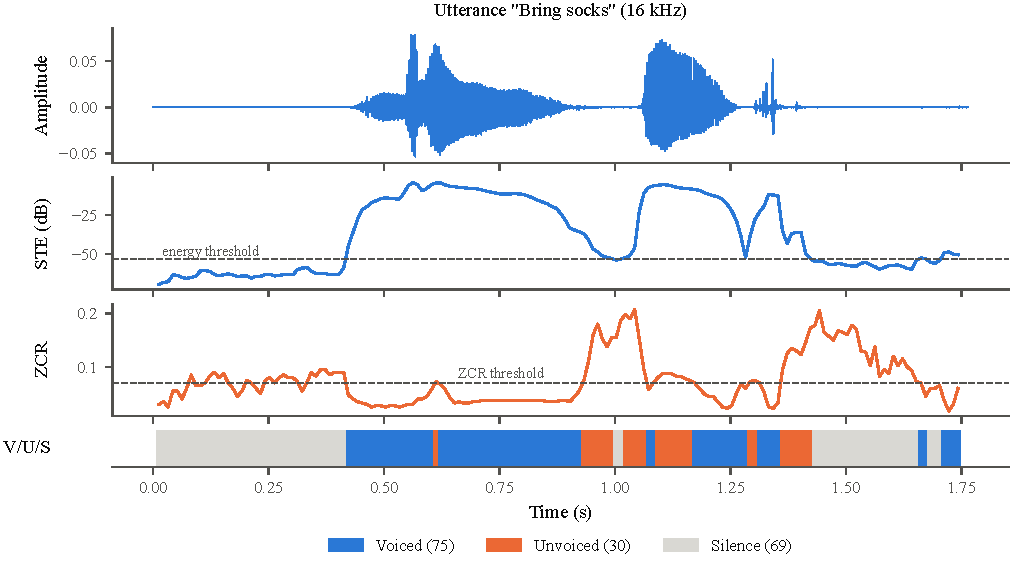
\includegraphics[width=0.80\textwidth]{fig_vus.pdf}\\[2pt]
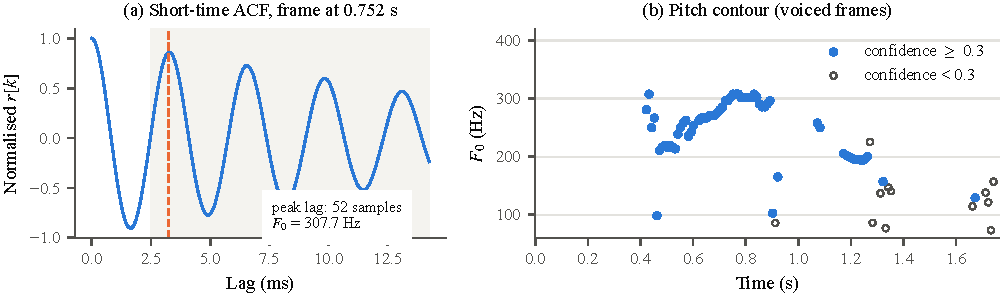
\includegraphics[width=0.80\textwidth]{fig_pitch.pdf}
\caption{Short-time analysis of \emph{``Bring socks''}. Top: waveform, short-time energy, zero-crossing rate and the voiced/unvoiced/silence labels. Bottom: (a) normalised autocorrelation of a voiced frame, with the 70--400~Hz search range shaded; (b) $F_0$ contour for each frame.}
\label{fig:vus}
\end{figure*}

The autocorrelation pitch analysis (Fig.~\ref{fig:vus}, bottom) gives an $F_0$ value for all 75 voiced frames, and 63 of them are above the confidence threshold. For the frame at 0.752~s, the autocorrelation has its peak at a lag of 52 samples ($F_0 = 307.7$~Hz), and there are more peaks at integer multiples of this lag. The pitch rises from about 210 to 310~Hz over \emph{``bring''} and falls from about 258 to 195~Hz over \emph{``socks''}. One value at 0.463~s (98.2~Hz, confidence 0.458) is close to half of the values around it. This is an octave error that still passes the confidence check. It shows that limiting the search range and checking the confidence reduce these errors, but they do not remove them fully~\cite{rabiner1977pitch}.

The spectrogram (Fig.~\ref{fig:spec}) is a separate way to check these results. In \emph{``bring''}, the harmonics are about 250--300~Hz apart, and this agrees with the autocorrelation result. The fricatives show energy spread over many frequencies with no harmonics, and the /k/ release shows up as a short vertical stripe across all frequencies. The narrowband (40~ms) analysis shows the separate harmonics. The wideband (5~ms) analysis shows the separate glottal pulses, but loses detail in frequency. The order-16 linear-prediction envelope of the frame at 0.752~s (Fig.~\ref{fig:spec}, bottom) shows two resonances, at 305 and 656~Hz. A second envelope calculated with Burg's method has both peaks at the same frequencies. The 305~Hz peak is close to the $F_0$ of this frame. It could be the first formant of the vowel in \emph{``bring''}; however, with only one frame, it is not possible to say whether a strong low harmonic at this high $F_0$ also adds to this peak. Lastly, the normalised autocorrelation of the residual at the pitch lag goes down from 0.406 at $p = 8$ to 0.346 at $p = 20$. This means that when the prediction order is higher, part of the periodicity of the source is taken into the all-pole filter.

\begin{figure*}[t]
\centering
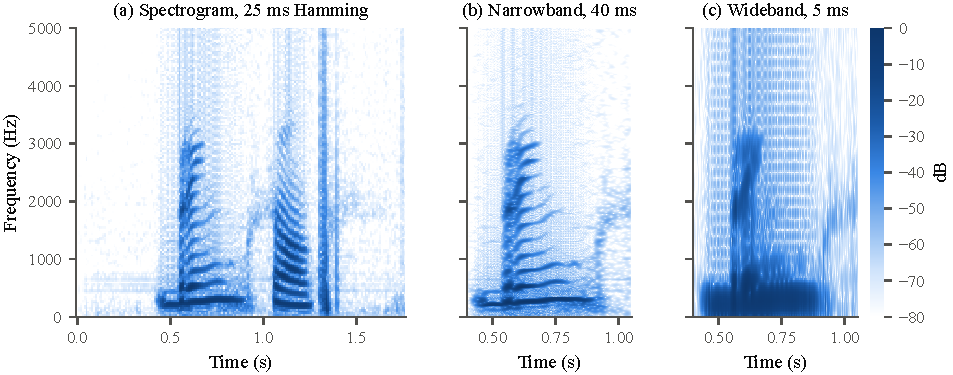
\includegraphics[width=0.80\textwidth]{fig_spectrogram.pdf}\\[2pt]
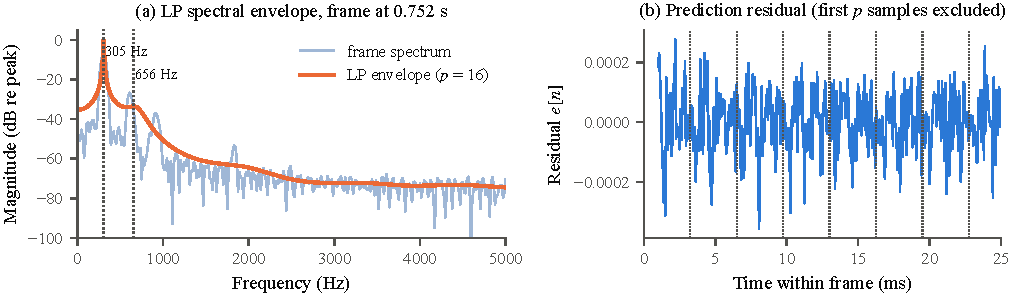
\includegraphics[width=0.80\textwidth]{fig_lpc.pdf}
\caption{Spectral analysis of \emph{``Bring socks''}. Top: (a) 25~ms Hamming spectrogram of the whole utterance; (b) narrowband and (c) wideband analysis of \emph{``bring''}. Bottom: (a) order-16 linear-prediction envelope over the spectrum of the frame at 0.752~s; (b) prediction residual, with dotted lines at multiples of the measured pitch period.}
\label{fig:spec}
\end{figure*}

\subsection{Tier 1: utterance-level statistics}
The results of the utterance-level classifiers are given in Table~\ref{tab:tier1}. With only the prosodic statistics, the tuned SVM gets 16.5\% on the test subset, which is 6.1 points above the majority baseline. For both classifiers, the accuracy stayed at around 15--16\% across all the hyperparameter settings. This shows that the problem is in the features and not in the classifier. Two patterns can be seen in the confusion matrix (Fig.~\ref{fig:cm1}). First, the most common intents get a large share of the predictions. For example, \emph{increase volume} makes up 20.3\% of the SVM's predictions, but only 10.4\% of the test labels. Second, the best-recognised intent, \emph{change language Chinese} (52.0\% recall), is mostly identified by its duration. Its phrasings are 3.06~s long on average, while the training average is 2.29~s. Eight intents are recognised at 1\% or less. Inverse-frequency class weighting increased the test macro-F1 of the SVM only from 0.115 to 0.120, and it brought the accuracy down to 12.2\%. Hence, it was not used.

\begin{table}[t]
\caption{Utterance-level classifiers, 31-class accuracy (\%): official partition and 5-fold speaker-grouped CV}
\label{tab:tier1}
\centering
\footnotesize
\setlength{\tabcolsep}{4pt}
\begin{tabular}{@{}llrrr@{}}
\toprule
Features & Classifier & Valid. & Test & CV\\
\midrule
-- & Majority class & 10.2 & 10.4 & $10.0 \pm 0.2$\\
Prosodic & SVM ($C{=}10$, $\gamma{=}0.01$) & 16.4 & 16.5 & $17.8 \pm 1.0$\\
Prosodic & MLP (64) & 15.2 & 14.3 & $16.5 \pm 1.5$\\
+ MFCC & SVM ($C{=}1$, $\gamma{=}0.01$) & 22.3 & \textbf{25.8} & $\mathbf{24.0 \pm 1.0}$\\
+ MFCC & MLP (64, 32) & 22.4 & 21.0 & $21.4 \pm 1.0$\\
\bottomrule
\end{tabular}
\end{table}

\begin{figure}[t]
\centering
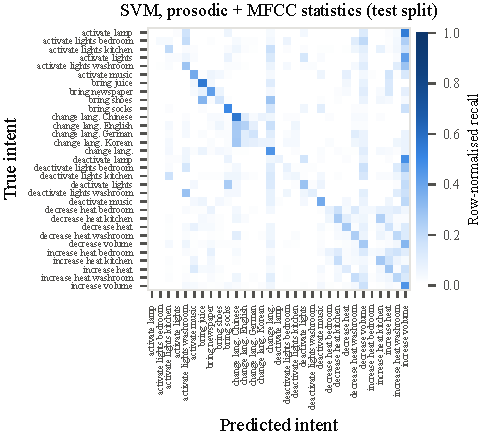
\includegraphics[width=\columnwidth]{fig_cm_svm_mfcc.pdf}
\caption{Row-normalised confusion matrix of the SVM on prosodic and MFCC statistics (official test subset, 25.8\% accuracy).}
\label{fig:cm1}
\end{figure}

When the MFCC statistics are added, the SVM goes up to 25.8\% (+9.3 points) and the MLP goes up to 21.0\% (+6.6 points). With speaker-grouped cross-validation, the same SVM settings give $17.8 \pm 1.0\%$ and $24.0 \pm 1.0\%$, and the MFCC statistics improve every fold (mean paired difference 6.2 points, $p < 0.001$). So the results on the official split also hold under the stricter protocol. This gain is bigger than any improvement that was obtained by tuning the prosodic system, and it matches the difference between the two types of features. Energy, ZCR, pitch, the two formants and the duration describe \emph{how} an utterance is spoken. The cepstral envelope, on the other hand, carries information about \emph{which} sounds are spoken, and it is these sounds that decide the intent. However, averaging over the utterance still loses the order in which the sounds occur. This limits what any static feature vector can do.

\subsection{Tier 2: classical sequence models}
The DTW 3-NN classifier gets 11.6\% on its 155 queries, and the per-class Gaussian HMM gets $6.0 \pm 0.7\%$ over the five folds. Both of these are close to or below the majority baseline. When the HMMs were trained and tested on the zero-padded sequences, the accuracy was $9.8\%$. The drop after the padding was removed shows that the padded version was partly using the amount of padding, which is a duration cue linked to the intent, and not the spectral information. After the padding was removed, the log-likelihood scores were finite and well separated, but a few of the class models won far more queries than they should have. These baselines were kept simple on purpose (three ergodic states, one Gaussian per state, no delta features and five DTW templates per class). Hence, the results show that such simple setups are not enough for 31 multi-word intents with 248 phrasings. They do not show that classical sequence models cannot work for this task in general.

\subsection{Tier 3: convolutional sequence models}
Table~\ref{tab:cv} gives a summary of the cross-validated models, grouped by tier. The single-head CNN on MFCC sequences gets $72.5 \pm 5.0\%$. This is three times the static MFCC result of Tier~1 on the same folds. Clearly, temporal order was the main thing missing in Tier~1.

\begin{table}[t]
\caption{Speaker-grouped five-fold cross-validation (full-intent accuracy, \%)}
\label{tab:cv}
\centering
\footnotesize
\begin{tabular}{@{}lrr@{}}
\toprule
Model & Mean $\pm$ s.d. & Range\\
\midrule
Prosodic + MFCC statistics + SVM (Tier 1) & $24.0 \pm 1.0$ & 22.7--25.2\\
\midrule
Gaussian HMM, MFCC & $6.0 \pm 0.7$ & 5.3--7.1\\
\midrule
1D-CNN, MFCC & $72.5 \pm 5.0$ & 65.4--77.6\\
1D-CNN, log-mel & $79.4 \pm 6.8$ & 70.9--88.5\\
Multi-head 1D-CNN, MFCC & $77.3 \pm 6.7$ & 67.6--83.3\\
\midrule
wav2vec 2.0 pooled + SVM & $59.9 \pm 4.4$ & 55.8--67.5\\
wav2vec 2.0 pooled + MLP & $69.9 \pm 4.7$ & 66.3--78.0\\
wav2vec 2.0 sequence + 1D-CNN & $\mathbf{93.1 \pm 3.1}$ & 88.9--96.9\\
\bottomrule
\end{tabular}
\end{table}

When the MFCC input is replaced with 40-band log-mel input in the same single-head network, the accuracy goes up to $79.4 \pm 6.8\%$. It improves in every fold (mean 6.9 points, $p = 0.005$). Both representations use the mel filter bank and the logarithm. MFCC also applies a DCT and keeps only 13 coefficients, and the log-mel input is also wider (40 dimensions instead of 13). To separate these factors, the DCT was applied to the same log-mel frames (Table~\ref{tab:dct}). When all 40 DCT coefficients are kept, no dimension is lost and the transform can be fully inverted, but the accuracy drops to $63.5 \pm 5.0\%$. This is 15.9 points below log-mel, and it is lower in every fold ($p < 0.001$). When the same transform is cut to 13 coefficients, the accuracy goes back up to $73.1 \pm 5.8\%$. This is almost the same as the original MFCC from 128 mel bands, and the difference is not significant ($p = 0.60$). Therefore, the log-mel input does better because the DCT is not applied, and not because it has more dimensions. Also, the number of mel bands makes no difference that can be measured.

\begin{table}[t]
\caption{Effect of the cepstral DCT on the 1D-CNN (31-class accuracy, \%, 5-fold speaker-grouped CV)}
\label{tab:dct}
\centering
\footnotesize
\begin{tabular}{@{}lcr@{}}
\toprule
Input (per frame) & Dim. & Mean $\pm$ s.d.\\
\midrule
40-band log-mel & 40 & $\mathbf{79.4 \pm 6.8}$\\
DCT of log-mel, first 13 coefficients & 13 & $73.1 \pm 5.8$\\
MFCC (128 mel bands), 13 coefficients & 13 & $72.5 \pm 5.0$\\
DCT of log-mel, all 40 coefficients & 40 & $63.5 \pm 5.0$\\
\bottomrule
\end{tabular}
\end{table}

The first convolutional layer could, in theory, learn to undo a transform that can be inverted. So the drop must come from the way the transformed input is given to the network. Before training, each input channel is standardised to unit variance. The standard deviations of the log-mel bands differ by a factor of 1.9; the standard deviations of the DCT coefficients differ by a factor of 60. Coefficients 14--40 carry only 2.2\% of the total variance. When the channels are standardised, these coefficients, which mostly describe fine spectral detail and noise, get the same weight as the coefficients that describe the spectral envelope. Truncation removes most of them, and this is why 13 coefficients do better than 40. The DCT is still useful for Gaussian models with diagonal covariance, because these models work better with decorrelated inputs. However, for the convolutional classifier used here, the log-mel input is the better choice. This agrees with what Mohamed \emph{et al.}~\cite{mohamed2012understanding} found.

After the input was fixed, the output structure was changed. When the MFCC network is split into action, object and location heads and trained with SpecAugment masking, the accuracy goes up to $77.3 \pm 6.7\%$. This is better than the single-head MFCC network in every fold (mean paired difference 4.8 points, $p = 0.007$). The accuracy for each slot is $85.3\%$ for the action, $91.7\%$ for the object and $94.1\%$ for the location (Fig.~\ref{fig:slots}). So the action slot is the weakest. Since this model also uses augmentation, the gain comes from both the split output and SpecAugment together. The single-head log-mel network and the multi-head MFCC network do not differ consistently (2.1 points in favour of log-mel, in 4 of 5 folds, $p = 0.16$). Hence, both changes give about the same benefit; using them together was not tested.

\begin{figure}[t]
\centering
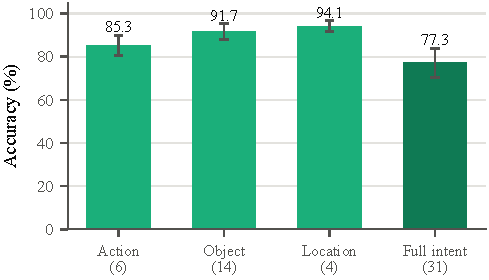
\includegraphics[width=0.85\columnwidth]{fig_multihead_slots.pdf}
\caption{Accuracy of the multi-head CNN for each slot and for the full intent (mean $\pm$ s.d. over folds; number of classes in brackets).}
\label{fig:slots}
\end{figure}

\subsection{Tier 4: frozen wav2vec 2.0 representation}
With mean pooling, the frozen wav2vec~2.0 representation gets $59.9 \pm 4.4\%$ with the SVM and $69.9 \pm 4.7\%$ with the MLP. These results are much higher than the static MFCC statistics of Tier~1. However, the pooled MLP is not significantly different from the MFCC CNN that was trained from scratch (mean paired difference $-2.6$ points, $p = 0.24$). This is because pooling loses the temporal order, just like the Tier~1 statistics. When the frame sequence is kept and classified by the network in Fig.~\ref{fig:cnn}, the accuracy goes up to $93.1 \pm 3.1\%$. This is higher than the log-mel CNN in every fold (mean paired difference 13.7 points, $p = 0.001$), and it also varies the least across folds out of all the models. Thus, the pooled and sequence results show two separate things. The pre-trained representation is the stronger feature when the temporal model is kept the same, but temporal modelling is still needed to make use of it.

The cross-validated accuracy of the frozen encoder is close to the 92.35\% that SUPERB reports for frozen wav2vec~2.0 Base on the official test split~\cite{yang2021superb}, even though the evaluation is done differently. It is still lower than the 98.8\% of the ASR-pre-trained model of Lugosch \emph{et al.}~\cite{lugosch2019fsc} and the 98.34\% of frozen HuBERT Base~\cite{yang2021superb}. The setup in this study uses only the final transformer layer, and this layer is known to have less phonetic information than the middle layers~\cite{pasad2021layerwise}. The PCA step also throws away 6.4\% of the variance. Both of these are likely reasons for the gap.

\subsection{Overall comparison}
All the 31-class results are shown on one axis in Fig.~\ref{fig:overall}, in order from classical to modern. Most of the progress comes from three steps. The first step is adding cepstral information to the utterance statistics (17.8 to 24.0\%). The second is keeping the temporal order with a convolutional network (24.0 to 72.5--79.4\%). The third is replacing the hand-crafted frame features with a frozen self-supervised representation (79.4 to 93.1\%). All the results except DTW use the same speaker folds; the DTW result is based on 155 queries from one fold. Also, the PCA in Tier~4 was fitted on utterances from the official training speakers, and some of these speakers are in held-out folds. Since the PCA does not use any labels and is very general, this effect is expected to be small. Even so, the PCA is not fitted separately inside each fold.

\begin{figure*}[t]
\centering
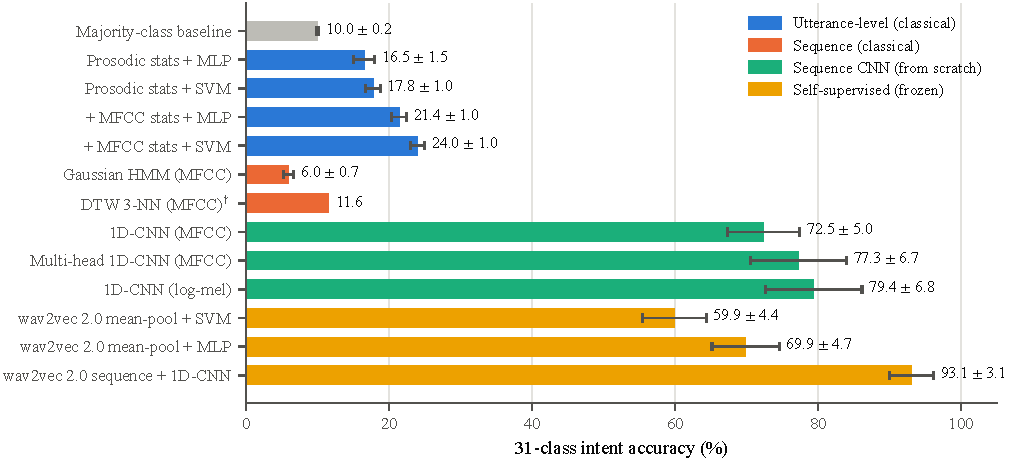
\includegraphics[width=0.80\textwidth]{fig_overall.pdf}\\[2pt]
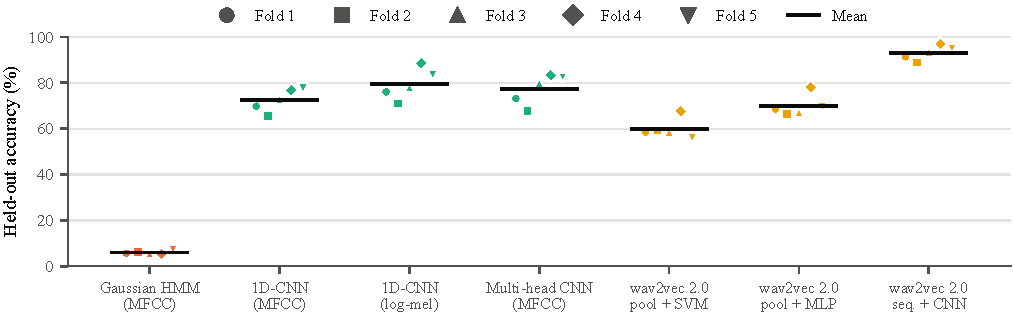
\includegraphics[width=0.80\textwidth]{fig_folds.pdf}
\caption{Top: intent accuracy of all the models with 5-fold speaker-grouped cross-validation, in order from classical to modern; the error bars show the standard deviation over folds ($^{\dagger}$DTW is evaluated on 155 queries from one fold). Bottom: held-out accuracy of each model in each fold, with horizontal bars at the mean.}
\label{fig:overall}
\end{figure*}

\subsection{Reduced-class slot tasks}
The three slot tasks from Section~\ref{sec:slots} are reported along with the 31-class task in Table~\ref{tab:slots} and Fig.~\ref{fig:slottasks}, using the same speaker folds. When the number of classes is reduced, every model gets a higher accuracy. For the SVM on prosodic and MFCC statistics, the accuracy goes up from 24.0\% on the intent to 40.7\% on the action, 49.3\% on the object and 64.3\% on the location. However, the majority-class baseline also goes up, from 10.0\% to 25.8\%, 31.2\% and 61.2\%, and most of the gain comes from this. To compare tasks that have different baselines, the fraction of the majority-class error that a model removes is used, $(a - a_{\mathrm{maj}})/(100 - a_{\mathrm{maj}})$. Using this, the SVM removes 15.6\% of the error on the intent, 20.1\% on the action, 26.3\% on the object and only 8.0\% on the location. On the location task, the MLP is actually below the baseline (60.5\% against 61.2\%). In most utterances, the location is not said at all. When it is said, it is a single word near the end of the command, and averages over the whole utterance do not capture this well.

\begin{table}[t]
\caption{Reduced-class slot tasks: mean accuracy (\%) over five speaker-grouped folds (number of classes in brackets)}
\label{tab:slots}
\centering
\footnotesize
\setlength{\tabcolsep}{4pt}
\begin{tabular}{@{}lrrrr@{}}
\toprule
Model & Loc.\ (4) & Act.\ (6) & Obj.\ (14) & Intent (31)\\
\midrule
Majority class & 61.2 & 25.8 & 31.2 & 10.0\\
Prosodic + SVM & 62.6 & 35.8 & 42.9 & 17.8\\
Prosodic + MFCC + SVM & 64.3 & 40.7 & 49.3 & 24.0\\
Prosodic + MFCC + MLP & 60.5 & 34.3 & 42.4 & 21.4\\
1D-CNN, log-mel & 90.6 & 85.1 & 89.1 & 79.4\\
wav2vec 2.0 + 1D-CNN & \textbf{97.5} & \textbf{95.1} & \textbf{96.4} & \textbf{93.1}\\
\bottomrule
\end{tabular}
\end{table}

\begin{figure*}[t]
\centering
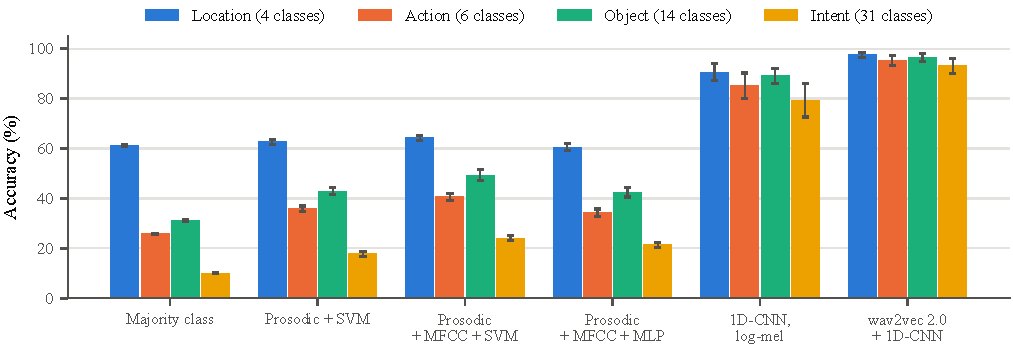
\includegraphics[width=0.80\textwidth]{fig_slot_tasks.pdf}
\caption{Accuracy on the three reduced-class slot tasks and on the 31-class intent task (mean $\pm$ s.d. over five speaker-grouped folds).}
\label{fig:slottasks}
\end{figure*}

The sequence models are quite different. The log-mel CNN gets 85.1--90.6\% on the slot tasks and the wav2vec~2.0 network gets 95.1--97.5\%. They remove 76--84\% and 92--95\% of the majority-class error, and this is about the same for every task. Therefore, using fewer classes does make the classical pipeline look better, but it does not change how it compares with the other tiers. The real problem is that the utterance-level features lose the temporal information; the number of classes is not the problem. It can also be seen that the single-slot log-mel networks are not better than the matching heads of the multi-head MFCC network (85.1, 89.1 and 90.6\% against 85.3, 91.7 and 94.1\% for the action, object and location). This suggests that training all the slots together, along with augmentation, helps each slot.

\subsection{Error analysis of the best model}
To look at the errors one by one, the wav2vec~2.0 sequence model was trained again on the first fold and its predictions were saved (91.7\% accuracy, compared with 91.4\% in the original run). The confusion matrix (Fig.~\ref{fig:cmw}) is mostly diagonal, and most of the errors that are left are between commands of opposite polarity. \emph{Increase volume} is predicted as \emph{decrease volume} 40 times. \emph{Increase heat} is predicted as \emph{decrease heat} in every location (8--14 times per location), and the same kind of confusion happens for the music and lamp commands. Because of this, the slot accuracy is lowest for the action (93.9\%), while it is 95.2\% for the object and 97.2\% for the location. In these phrasings, the polarity is often given by one short, unstressed word such as \emph{up}/\emph{down} or \emph{on}/\emph{off}, while the rest of the command is the same. So one small acoustic cue decides the label. The accuracy also changes a lot between the 19 held-out speakers: 14 of them are above 89\%, while two of them are recognised at only 36.4\% and 44.2\%. This variation between speakers explains why the results change across folds in Table~\ref{tab:cv}, and why the official split with ten speakers is not stable.

\begin{figure}[t]
\centering
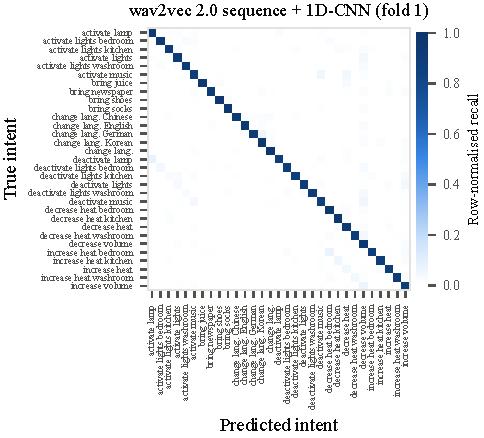
\includegraphics[width=\columnwidth]{fig_cm_w2v.pdf}
\caption{Row-normalised confusion matrix of the wav2vec~2.0 sequence model on the held-out speakers of fold 1 (91.7\% accuracy).}
\label{fig:cmw}
\end{figure}

%=====================================================================
\section{Conclusion}\label{sec:conclusion}
%=====================================================================
In this study, spoken intent classification on Fluent Speech Commands was studied using different speech representations, from classical short-time analysis to a frozen self-supervised encoder. The classical feature-extraction pipeline worked as expected on individual utterances, and the pitch, spectral and linear-prediction results agreed with each other. However, prosodic statistics of the utterance carry very little of the information needed to tell the intents apart ($17.8\%$ with cross-validation), and cepstral statistics only recover part of it ($24.0\%$). The simple DTW and HMM baselines did not do better than the majority class. Convolutional networks trained from scratch on frame sequences increased the accuracy to 72.5--79.4\%. Out of these, log-mel input did better than MFCC in every fold. This is because the cepstral DCT, along with per-channel standardisation, gives too much weight to the low-variance coefficients. The same network on frozen wav2vec~2.0 frames reached 93.1\%.

Over the whole study, keeping the temporal order gave the biggest gain, and the pre-trained representation gave the second biggest gain. Reducing the task to the action, object or location slot increased the accuracy of every model. However, the utterance-level statistics removed at most a quarter of the majority-class error on any slot, while the sequence models removed 76--95\%. Hence, the number of classes is not the main problem for the classical pipeline. The errors that remain in the best model are mostly between commands of opposite polarity, and on a few hard speakers. The evaluation also showed that the official FSC subsets, with only ten speakers each, are too small to give stable results on a single split. Speaker-grouped cross-validation with paired comparisons is a more reliable way to compare models on this corpus.

This work can be extended in a few ways. Classical sequence baselines with a left-to-right topology, Gaussian mixtures and delta features~\cite{furui1986delta} would give a fairer classical comparison. For the self-supervised tier, the next steps would be a learned weighting of the encoder layers~\cite{yang2021superb}, a comparison with HuBERT~\cite{hsu2021hubert} and fine-tuning of the encoder. Testing with added noise and on phrasings that were not seen in training would also be useful.

\section*{Acknowledgment}
The authors would like to thank Dr.~Jyothish Lal for the guidance provided throughout this course project.

\bibliographystyle{IEEEtran}
\bibliography{refs}

\end{document}
